\documentclass[12pt,a4paper]{article}
\usepackage[margin=2cm]{geometry}
\usepackage{graphicx} % Required for including pictures
\usepackage{float} % Allows putting an [H] in \begin{figure} to specify the exact location of the figure
\usepackage{wrapfig} % Allows in-line images such as the example fish picture
\usepackage{color}
\usepackage{mathtools} 
\usepackage{hyperref} % Fancy hyperrefs
\usepackage{titling} % Lets us compactify our heading
\usepackage{braket} % ???
\usepackage{cancel} % ???
\usepackage{acronym} % Acronym Package$
\usepackage{subcaption} % Captions for subfigures %
\usepackage{caption} % Caption subtlety
\usepackage[space]{grffile} % allows file names with spaces
\usepackage{lipsum} % Allows for placeholder text

\hypersetup{
colorlinks=true,
linkcolor=blue,
urlcolor=blue
}

\acrodef{stem}[STEM]{Scanning Transmission Electron Microscopy}
\acrodef{tem}[TEM]{Transmission Electron Microscope}
\acrodef{cemn}[CEMN]{Center for Electron Microscopy and Nanofabrication}
\acrodef{edx}[EDX]{Energy-dispersive X-ray spectroscopy}
\acrodef{sem}[SEM]{Scanning Electron Microscope}
\acrodef{psu}[PSU]{Portland State University}
\acrodef{hr}[HRTEM]{High Resolution \ac{tem}}
\acrodef{al}[$Al$]{Aluminum}
\acrodef{si}[$Si$]{Silicon}
% http://staff.science.uva.nl/~polko/HOWTO/LATEX/acronym.html 

%\setlength\parindent{0pt} % Uncomment to remove all indentation from paragraphs

\graphicspath{{Data/}} % Specifies the directory where pictures are stored

\title{TEM Report 3}
\author{Bret Comnes}
\date{\today}
\posttitle{\par\end{center}}
\setlength{\droptitle}{-10pt}


\begin{document}

\maketitle

\section{Introduction} % Major section

This report will focus on the the analysis of the diffraction patterns that were acquired in the \ac{cemn} at \ac{psu} on May 23rd, 2014.  Diffraction pattern, Kikuchi pattern and \ac{hr} images were acquired using an FEI Technai \ac{tem}.

This paper will cover a brief conceptual/theoretical description of diffraction pattern formation.  We will then analyze diffraction patterns of a \ac{al} polycrystalline sample and a single-crystalline \ac{si} sample.  We will also analyze the lattice structure and spacing of a gold foil sample using a \ac{hr} image taken of the sample.  A Kikuchi pattern is also included and briefly discussed.

\section{Diffraction Pattern Formation} % (fold)
\label{sec:diffraction_pattern_formation}

\lipsum[20]

% section diffraction_pattern_formation (end)

\subsection{Aluminum Polycrystalline Diffraction Pattern} % (fold)
\label{sub:poly}

\lipsum[20]

\begin{figure}[htbp]
  \centering
    \begin{subfigure}[b]{0.45\textwidth}
    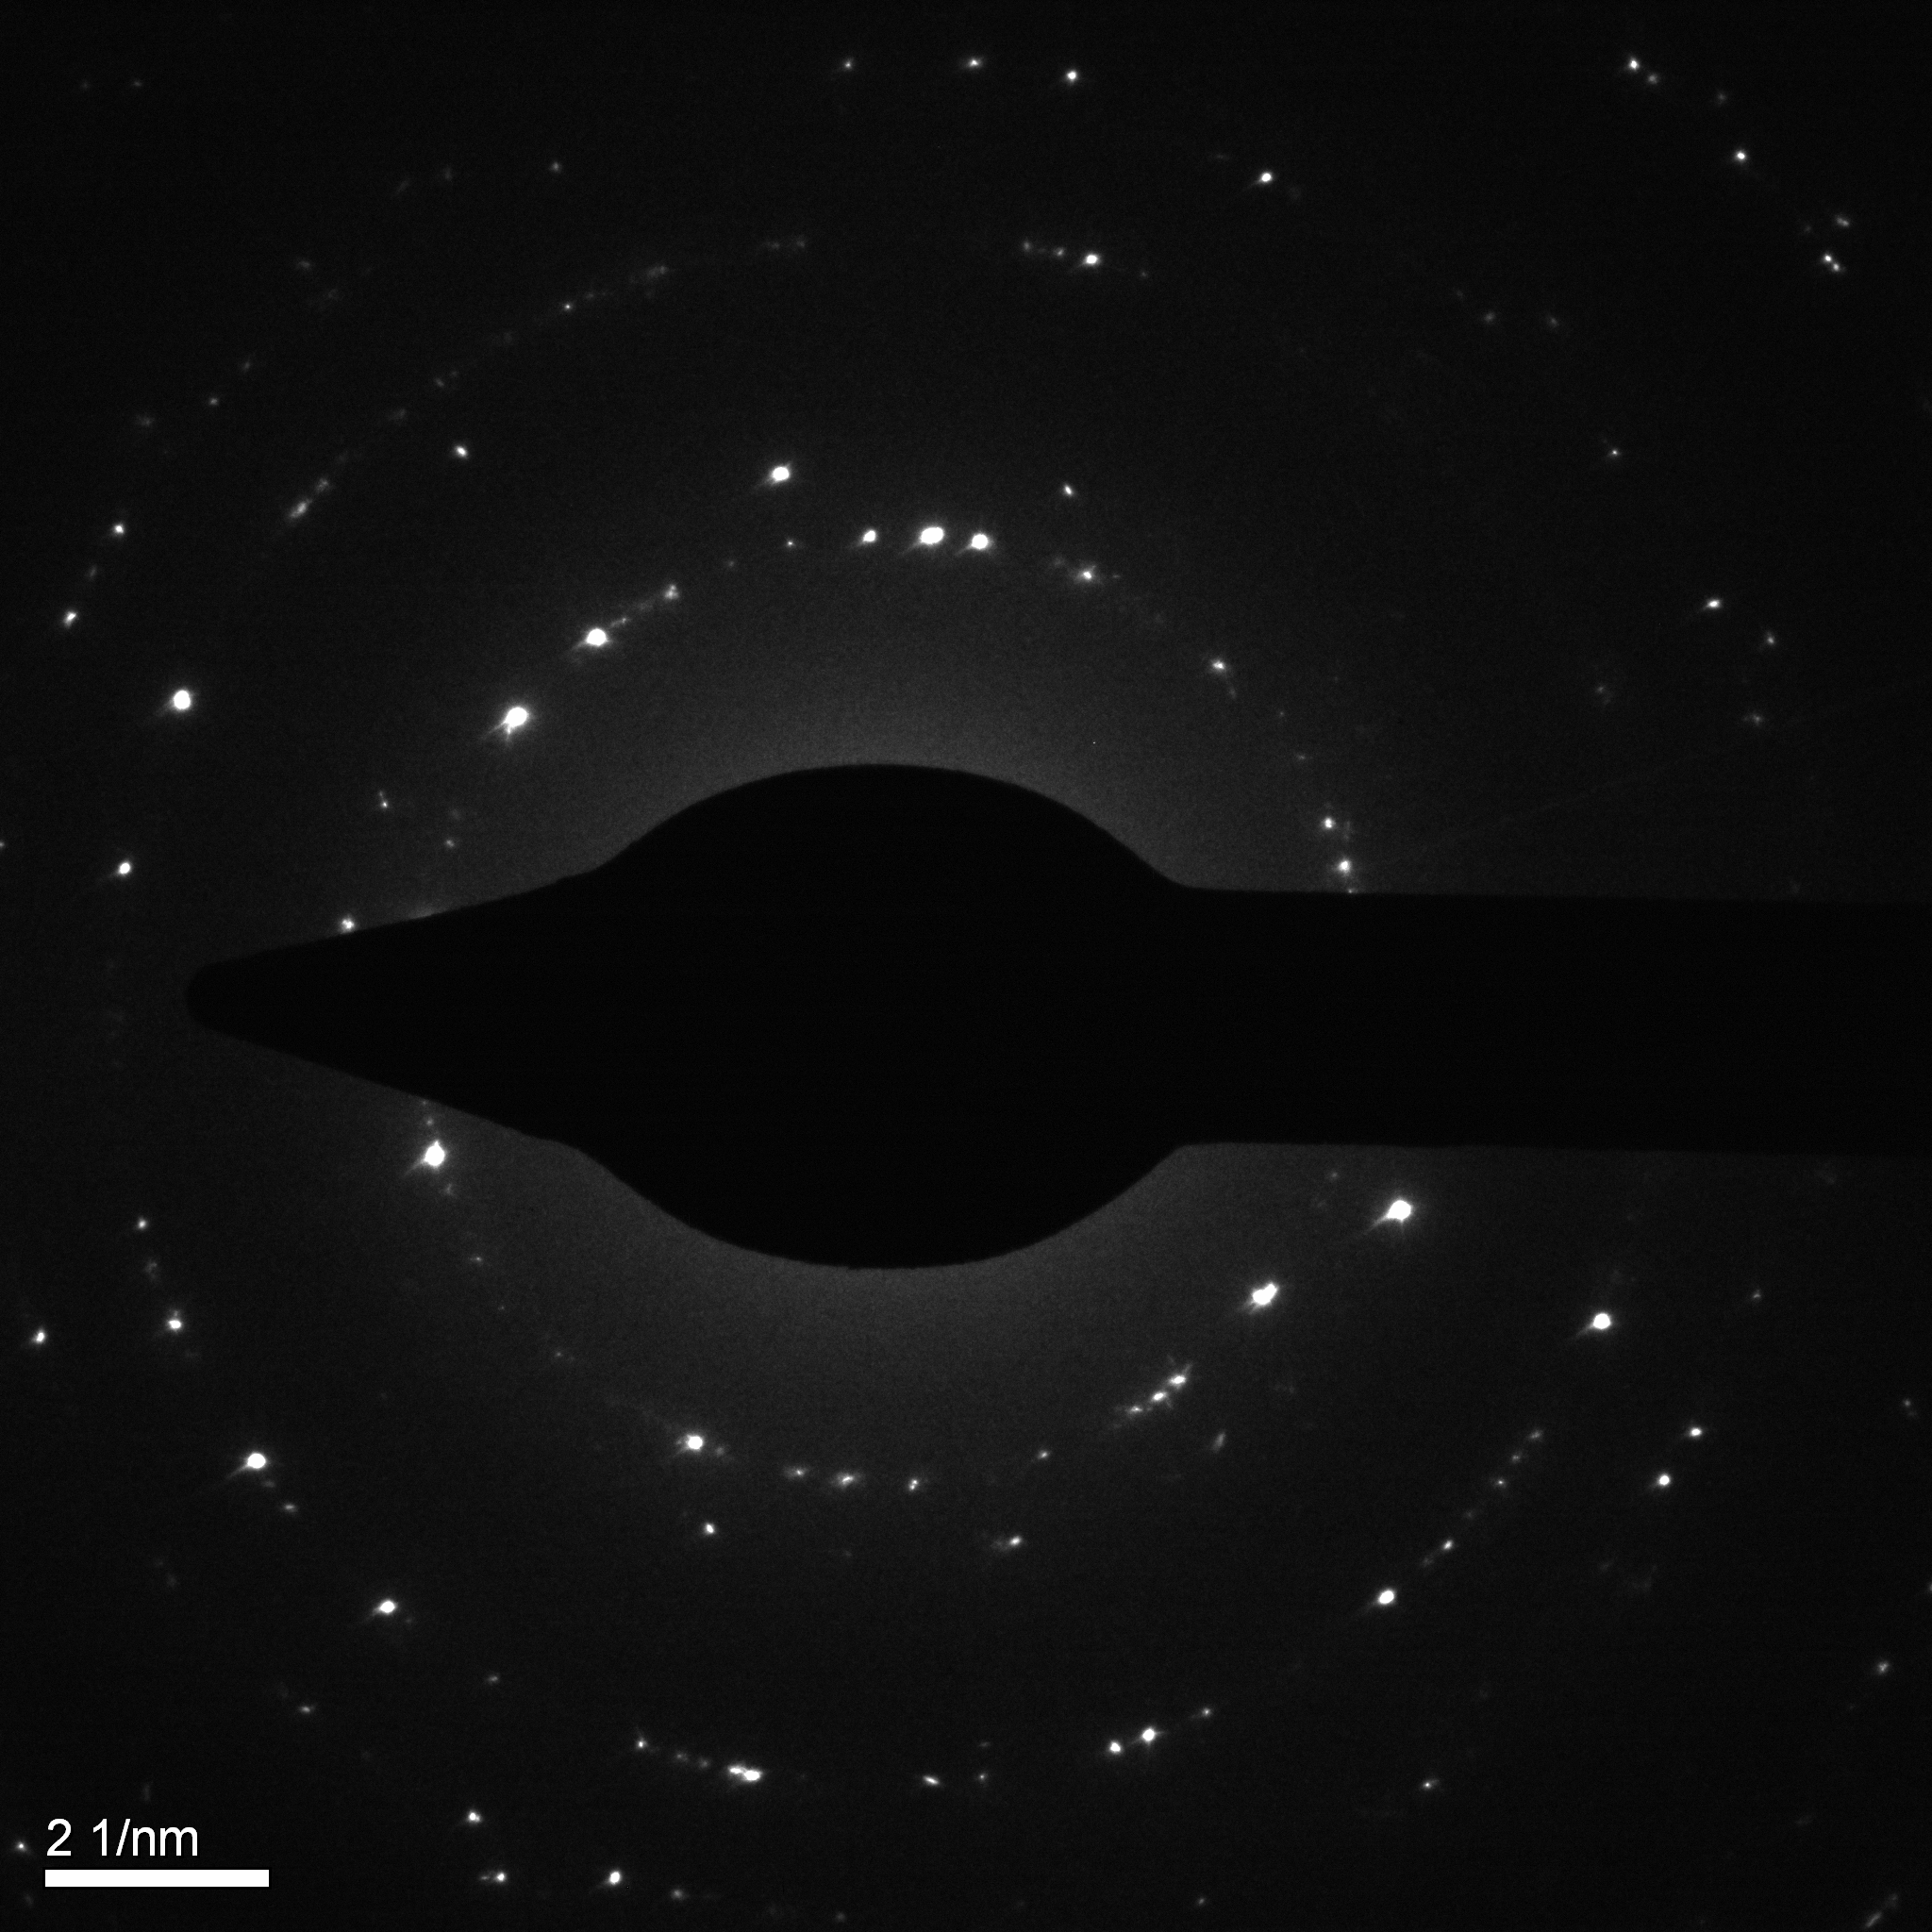
\includegraphics[width=\textwidth]{data/Image1 Al_Diff_SAED2.png}
    \caption{aluminum polycrystalline pattern using SAED setting 2}
    \label{fig:al2}
  \end{subfigure}%
  ~
  \begin{subfigure}[b]{0.45\textwidth}
    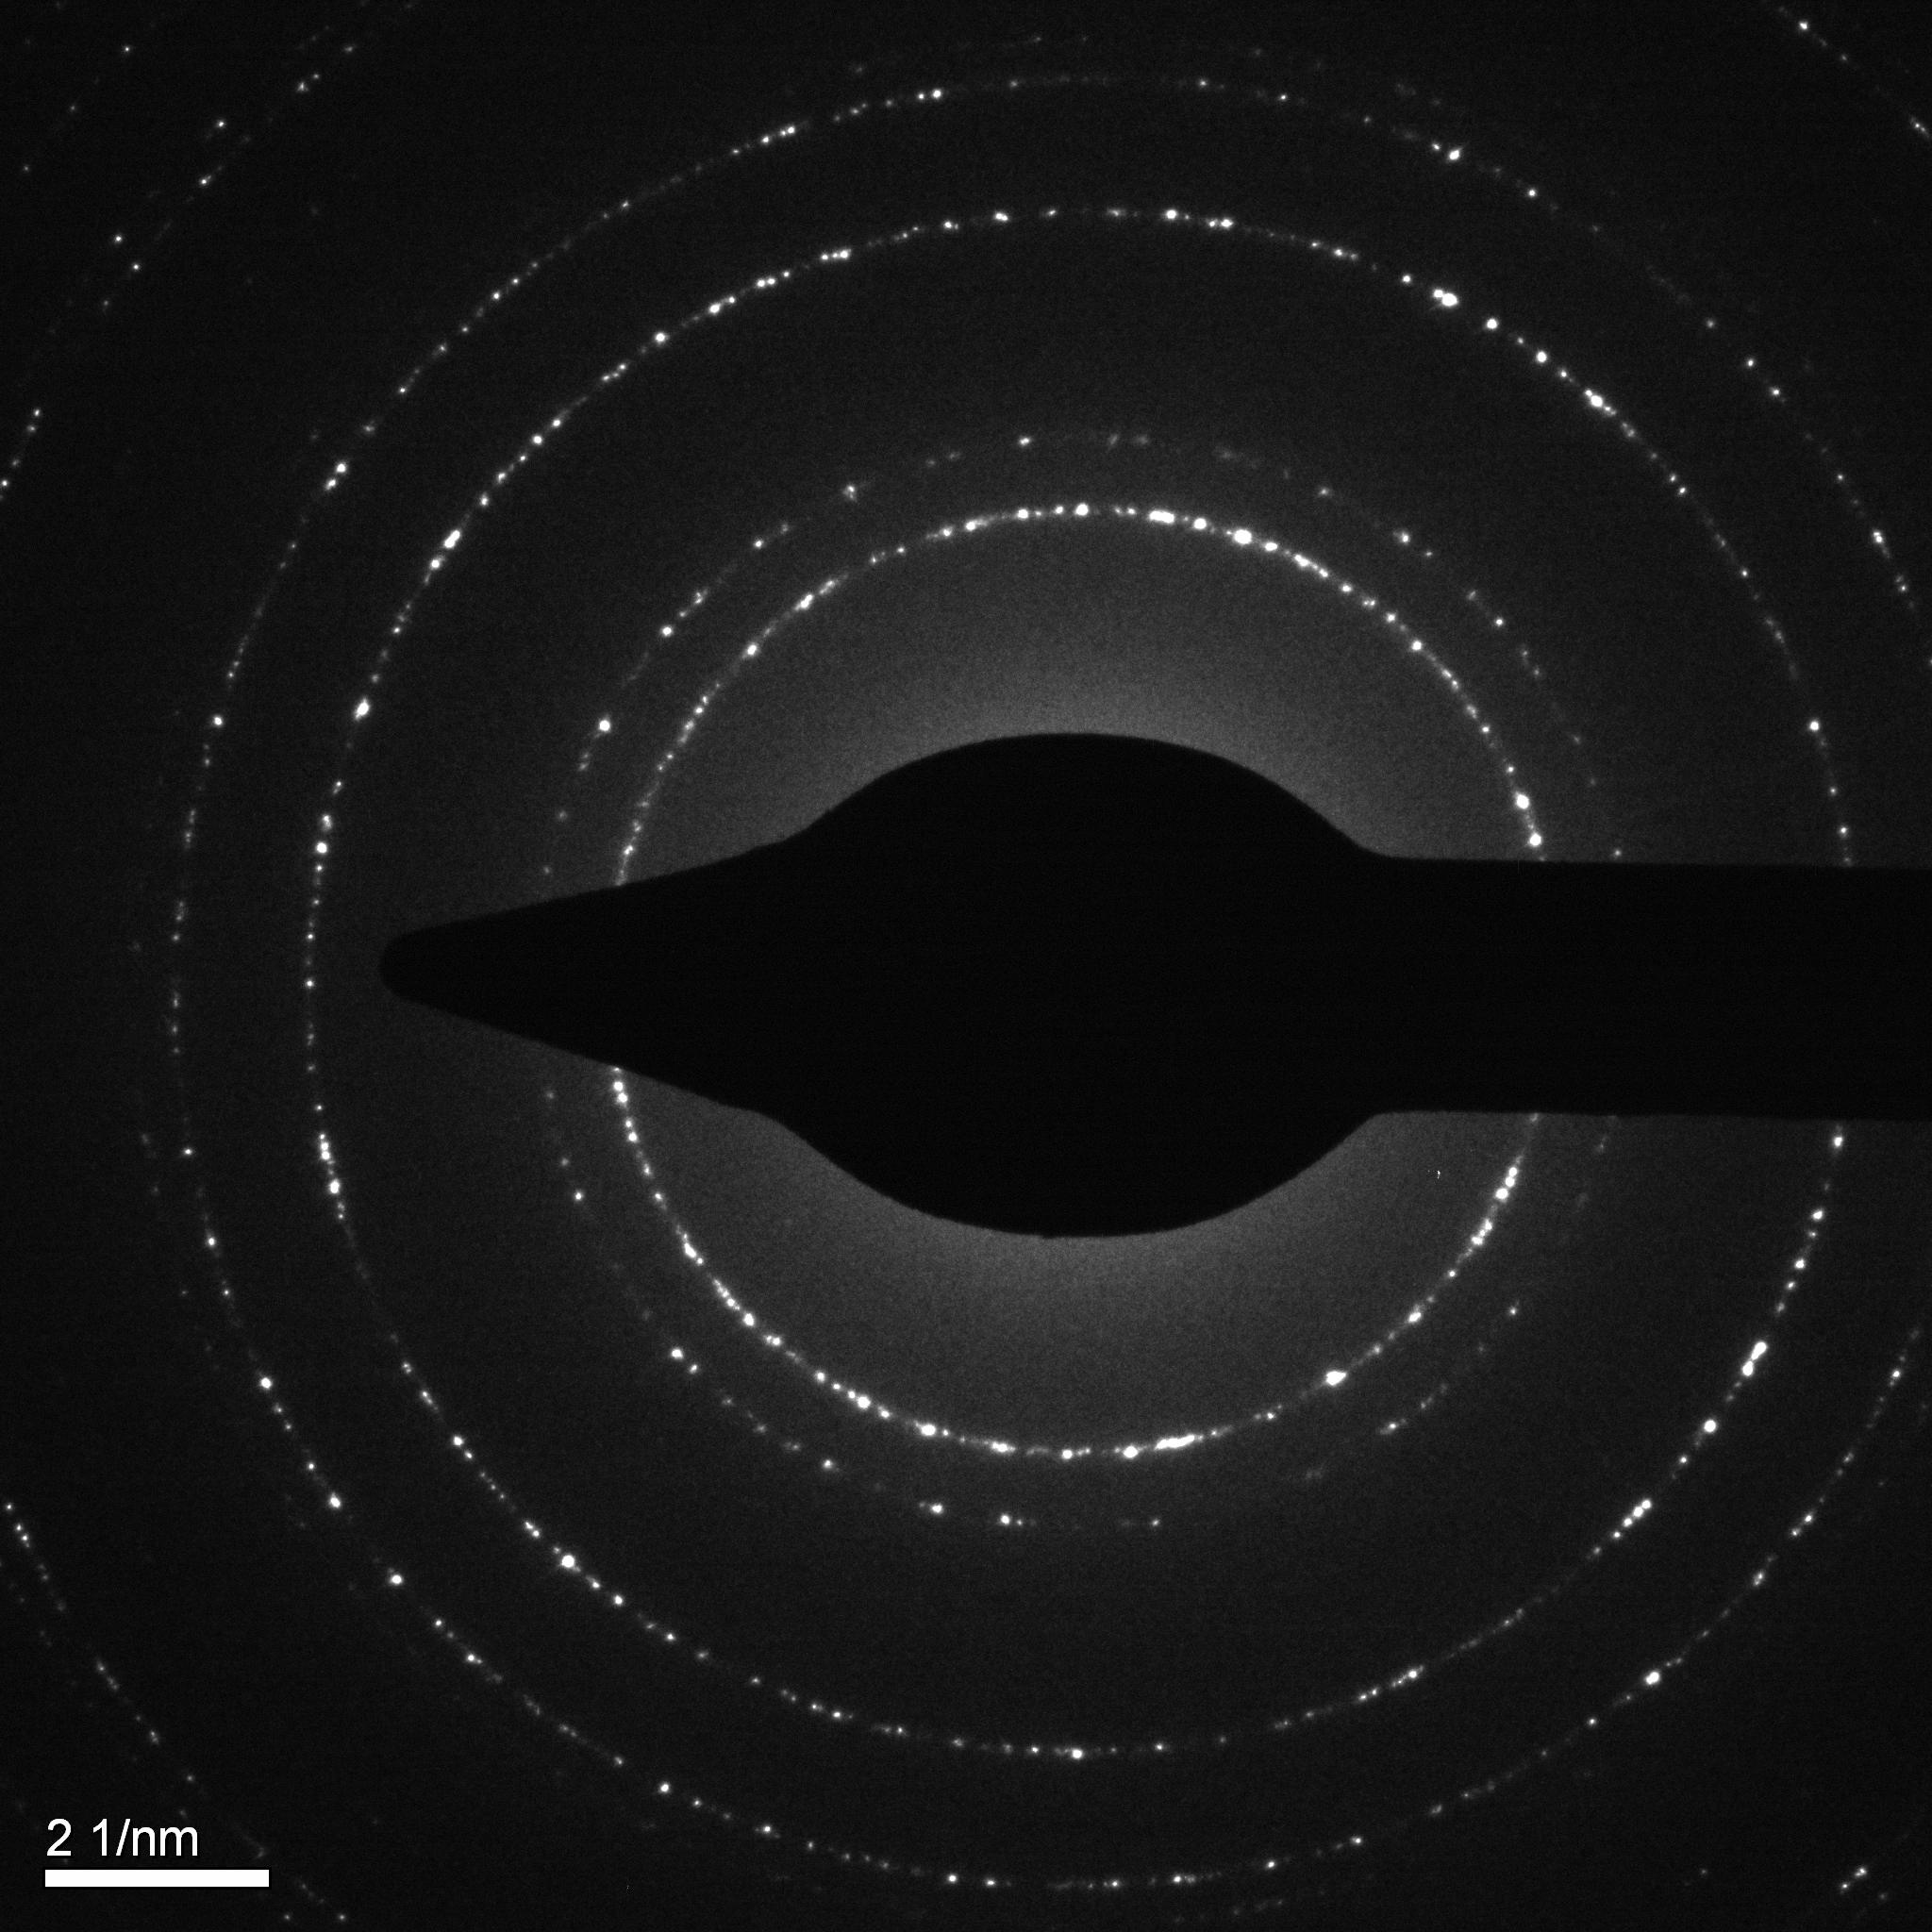
\includegraphics[width=\textwidth]{data/Image2Al_Diff_SAED3.png}
    \caption{aluminum polycrystalline pattern using SAED setting 3, }
    \label{fig:al3}
  \end{subfigure}
  \caption{Aluminum Polycrystalline Diffraction Pattern}
  \label{fig:aluminum}
\end{figure}

% subsection ac (end)

\subsection{Single-Crystalline Silicon Diffraction Pattern} % (fold)
\label{sub:single_crystaline}

\lipsum[20]

\begin{figure}[htbp]
  \centering
    \begin{subfigure}[b]{0.45\textwidth}
    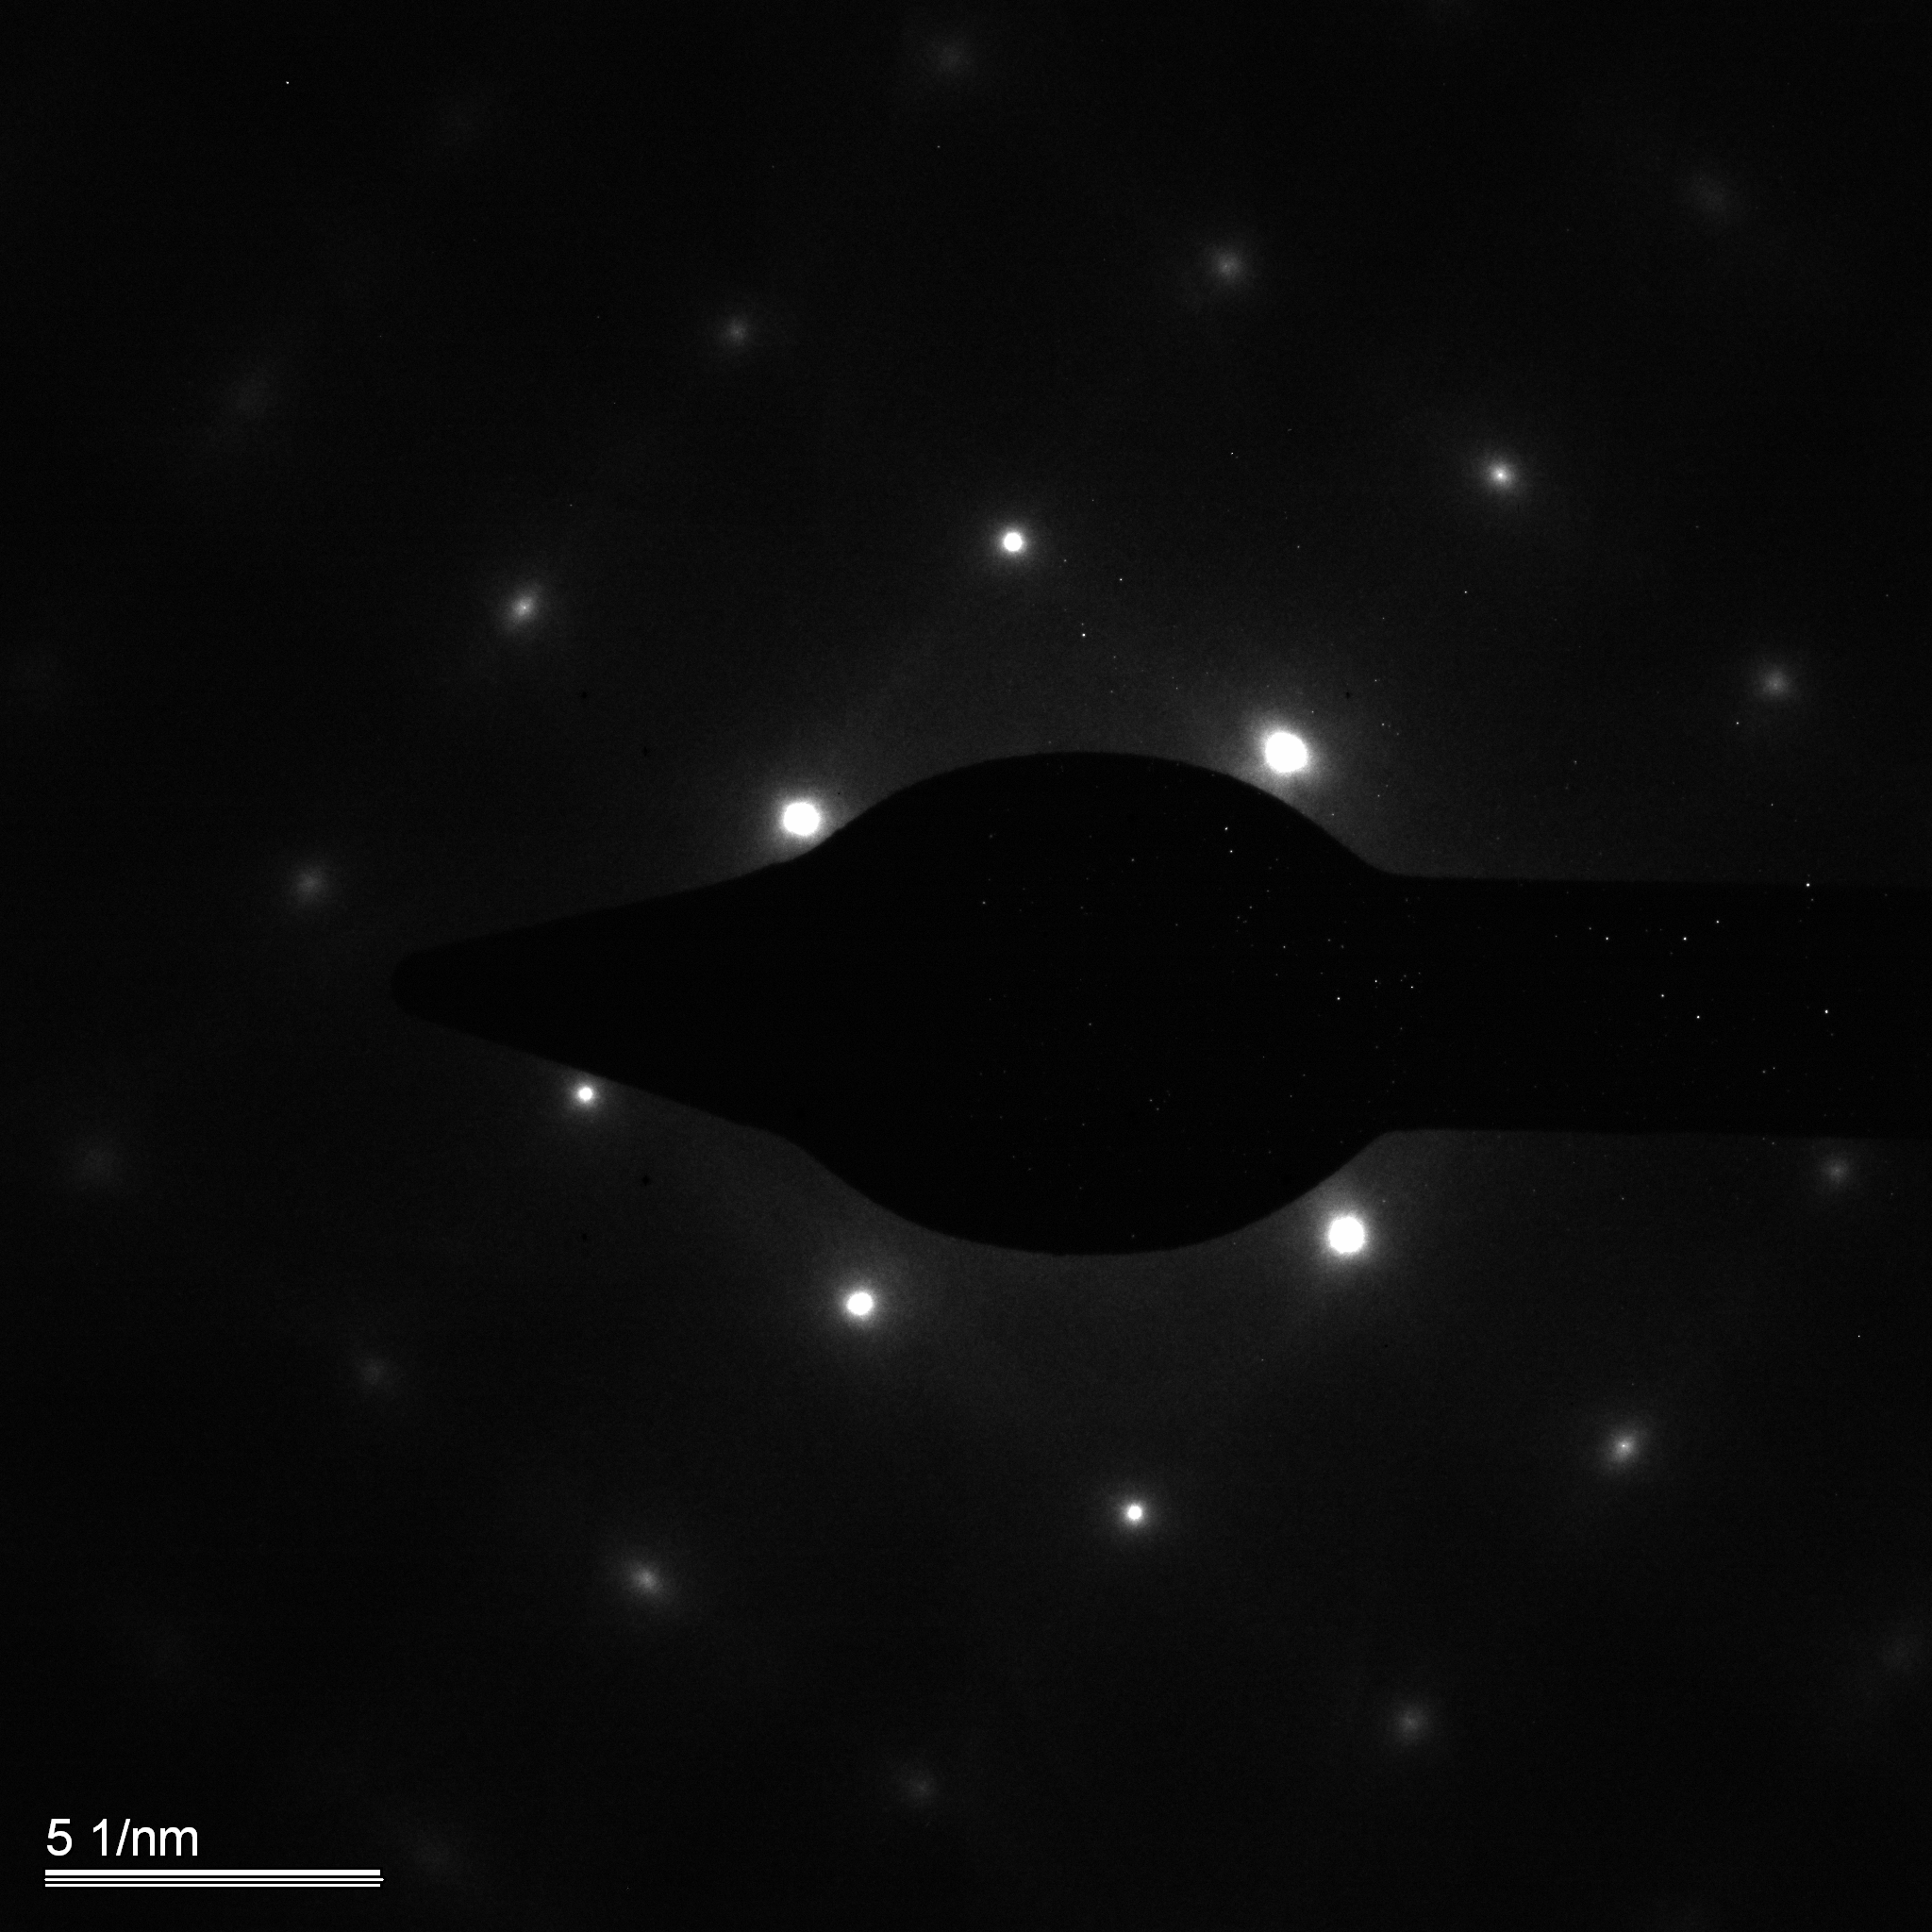
\includegraphics[width=\textwidth]{data/Image3 Si_Diff_Zone1.png}
    \caption{single-crystalline silicon pattern at one zone axis}
    \label{fig:si1}
  \end{subfigure}%
  ~
  \begin{subfigure}[b]{0.45\textwidth}
    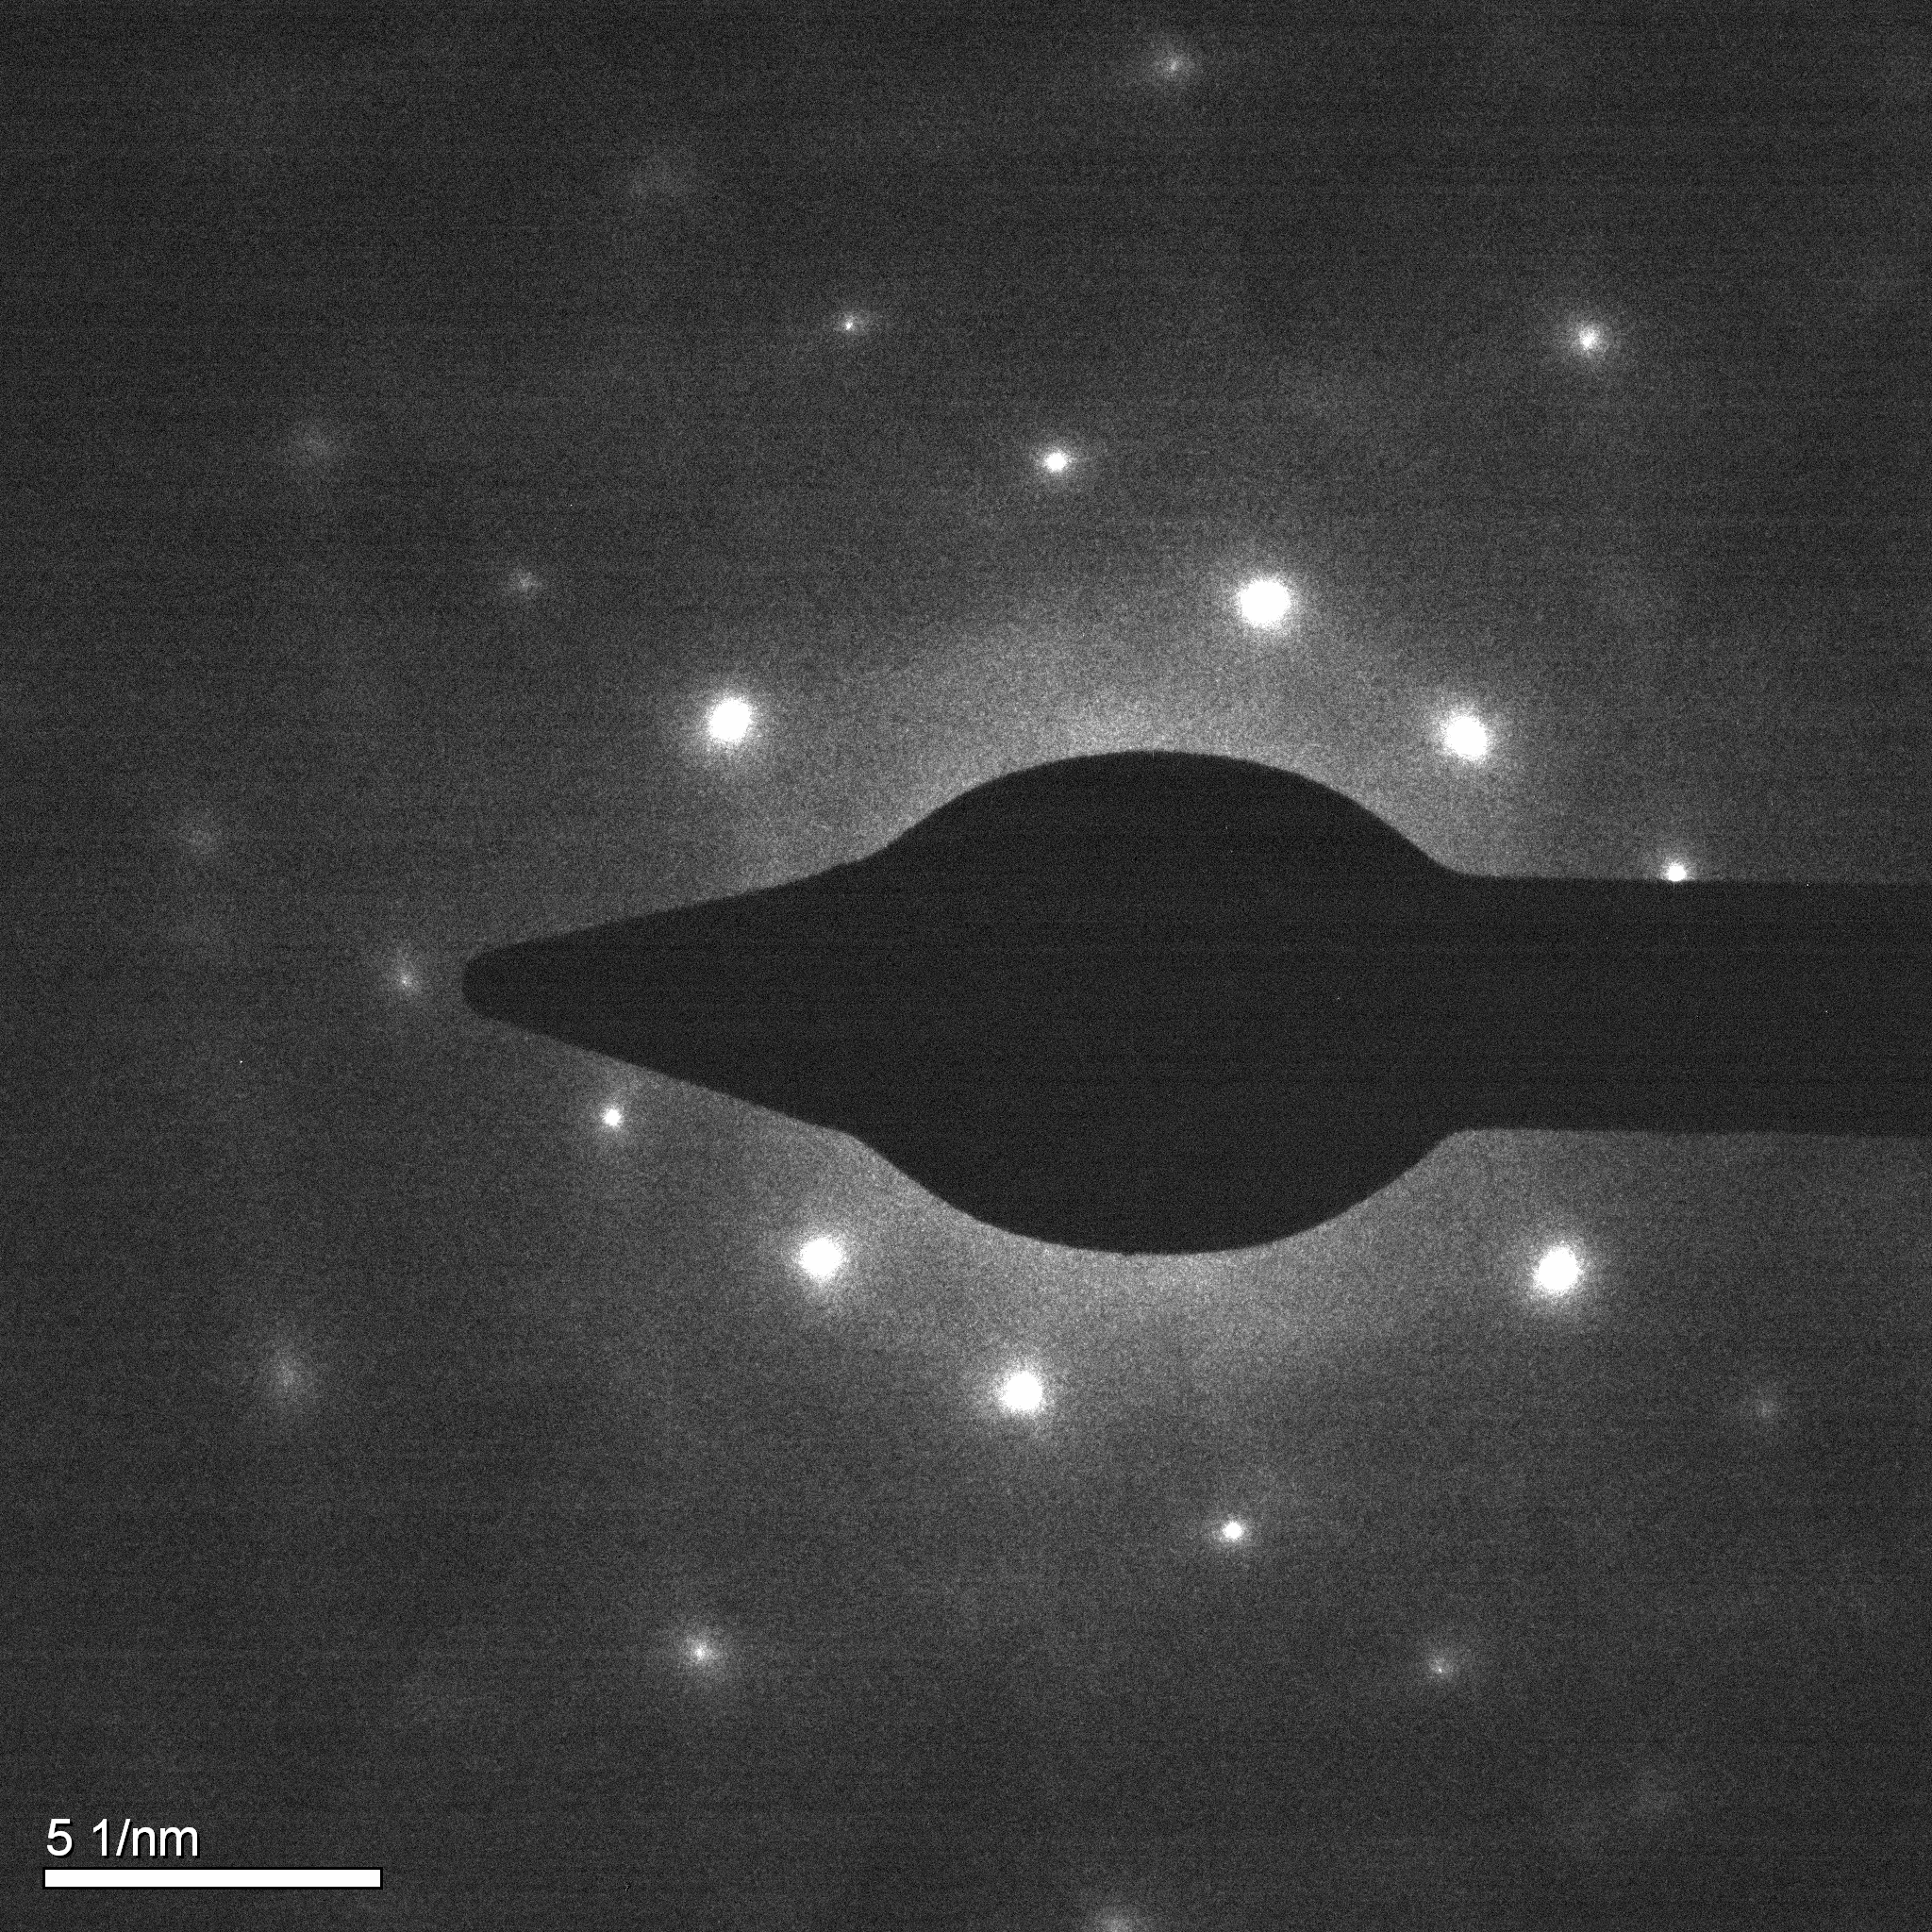
\includegraphics[width=\textwidth]{data/Image4 Si_Diff_Zone2.png}
    \caption{single-crystalline silicon pattern at another zone axis}
    \label{fig:si2}
  \end{subfigure}
  \caption{Single-Crystalline Silicon Diffraction Pattern}
  \label{fig:Silicon}
\end{figure}

% subsection single_crystaline_ac (end)

\subsection{Silicon Kikuchi Pattern} % (fold)
\label{sub:kikuchi_pattern}

\lipsum[20]

\begin{figure}[htbp]
  \centering
  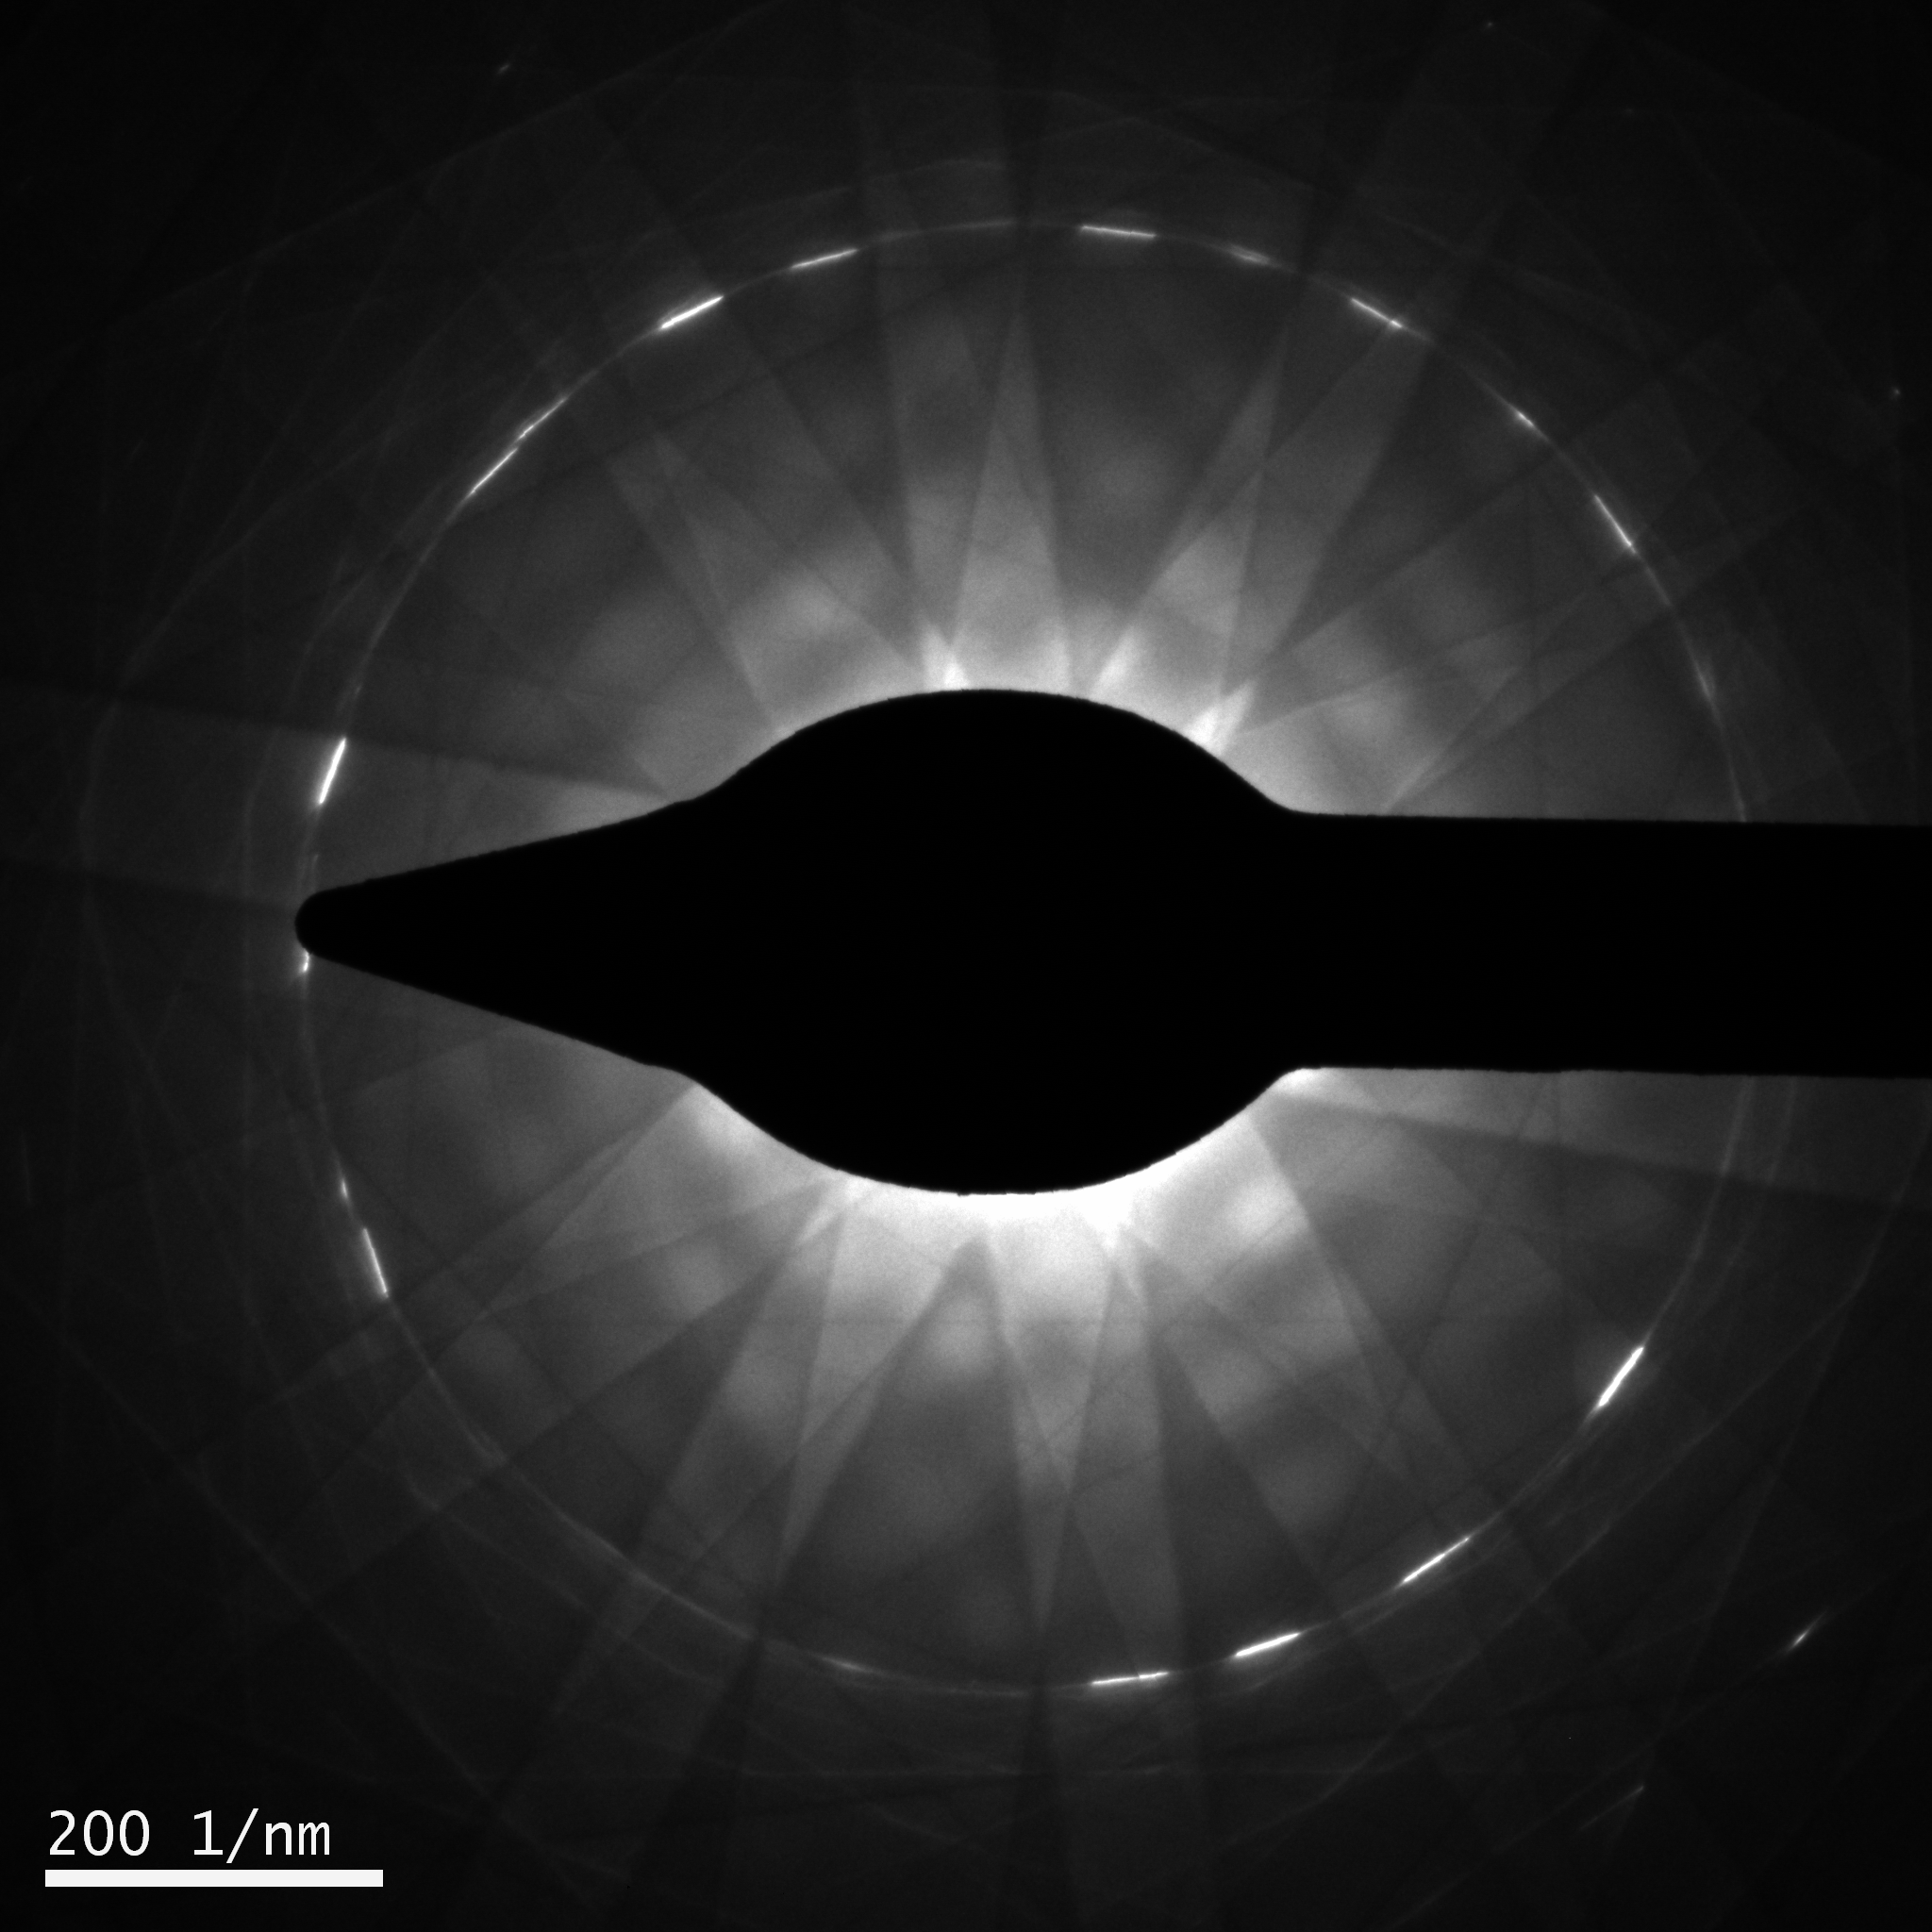
\includegraphics[width=0.95\textwidth]{data/Image6 Si_Kikuchi.png}
  \caption{Silicon Kikuchi pattern}
  \label{fig:kikuchi}
\end{figure}

% subsection ackikuchi_pattern (end)

\section{Lattice Structure Fundamentals} % (fold)
\label{sec:lattice_structure_fundamentals}

\lipsum[20]

\subsection{Lattice Spacing of Gold Foil Sample} % (fold)
\label{sub:lattice_spacing_of_gold_foil_sample}

\lipsum[20]

\begin{figure}[htbp]
  \centering
  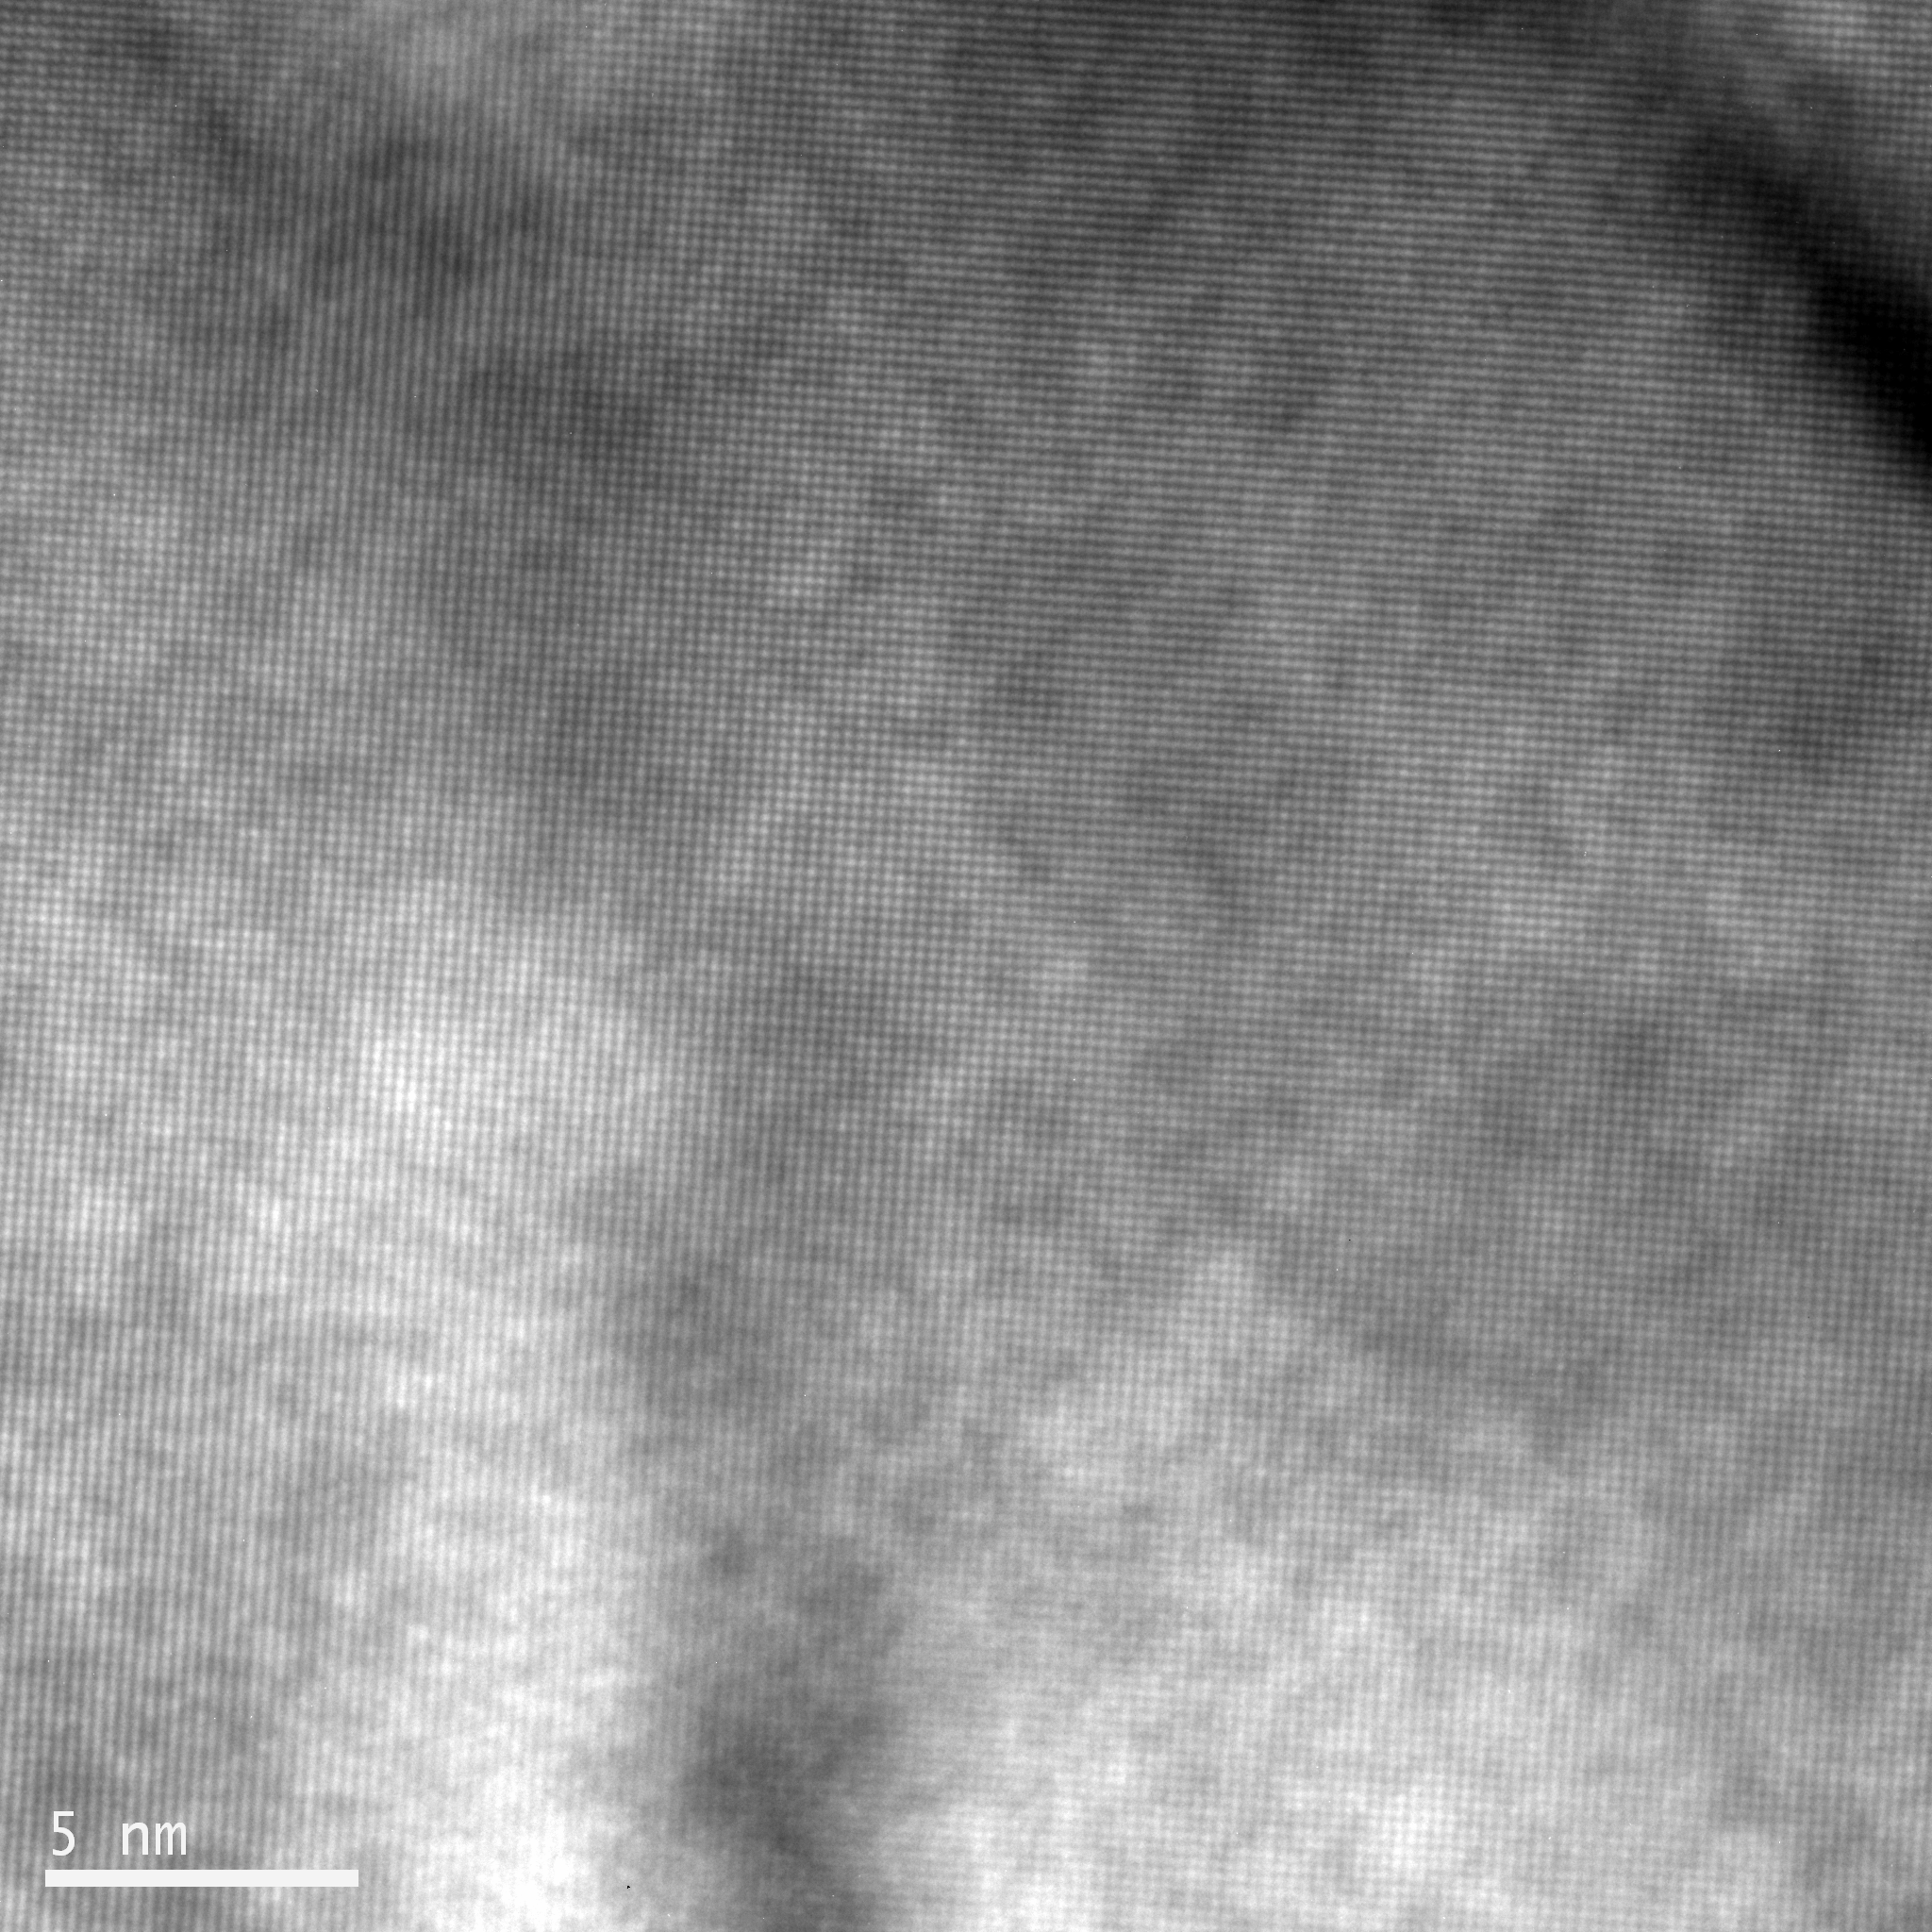
\includegraphics[width=0.95\textwidth]{data/Image5 Au_HRTEM.png}
  \caption{Al \ac{hr} image}
  \label{fig:hr_au}
\end{figure}

% subsection lattice_spacing_of_gold_foil_sample (end)

% section lattice_structure_fundamentals (end)

\section{Conclusion} % Major section



\bibliography{references-3} 
\bibliographystyle{plain} \nocite{*}

\end{document}